\documentclass[onecolumn]{article}
%\usepackage{url}
%\usepackage{algorithmic}
\usepackage[a4paper]{geometry}
\usepackage[margin=2em, font=small,labelfont=it]{caption}
\usepackage{graphicx}
\usepackage{mathpazo} % use palatino
\usepackage[scaled]{helvet} % helvetica
\usepackage{microtype}
\usepackage{amsmath}
\usepackage{subfigure}
% Letterspacing macros
\newcommand{\spacecaps}[1]{\textls[200]{\MakeUppercase{#1}}}
\newcommand{\spacesc}[1]{\textls[50]{\textsc{\MakeLowercase{#1}}}}

\title{\spacecaps{Fake News Detection}\\ \normalsize \spacesc{using Scikit-Learn} }

\author{Murat Doğan\\muratdogan5@posta.mu.edu.tr}


\begin{document}
\maketitle

\section{Introduction}
Fake news is one of the biggest problem of this century. This project includes detecting fake news deals with fake and real news using different algoritms and includes comparing these algoritms by looking accuracy scores and confusion matrices

\section{Detecting fake news with scikit learn}


\subsection{Import Libraries}
In this project, I used;\newline
-sklearn for data processing,\newline
-matplotlib, pandas for visualization our data and results.\bigskip\newline
\noindent
To import these libraries, I used "import" statement (e.g "import matplotlib.pyplot").

\subsection{Import Dataset}
The dataset which will use, has 6335 rows x 4 columns. These columns are id, title, text and label. Title is heading of news, text is content of the news and label is news label is whether the news is fake or real\bigskip\newline
\noindent
To implement my dataset, I used "read\_csv" function from pandas.\bigskip\newline
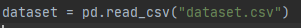
\includegraphics{fig/d.PNG}


\subsection{Visualization of Dataset}
How many fake and real news in dataset? To know, I grouped using ".groupby()", ".count()" for size and ".plot()" for plotting\bigskip\newline
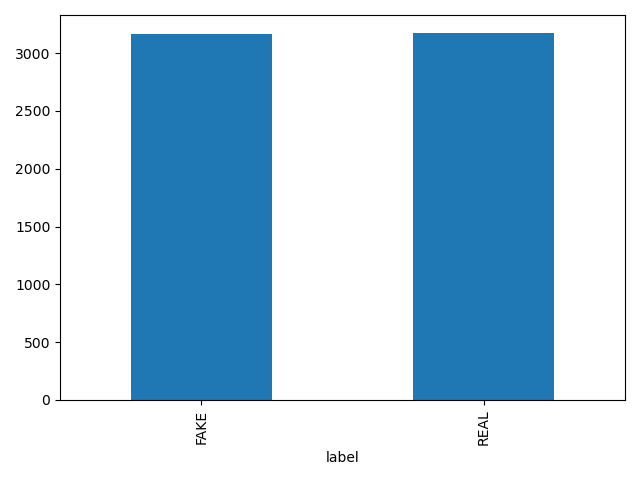
\includegraphics[scale=0.3]{fig/count.PNG}
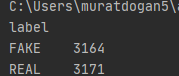
\includegraphics[scale=1]{fig/count2.PNG}

\subsection{Prepare Dataset}
First of all, I need to find accuracy value for find the algorithm is efficient. I should split my data to train and test part. To do this, I used "train\_test\_split" function. X value is my content of news, y value is label and test data ratio is 0.3
\bigskip\newline
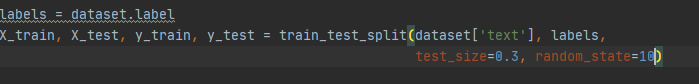
\includegraphics[scale=0.7]{fig/3.PNG}

\subsection{Vectorizers}
Text data requires special preparation before you can start using it for predictive modeling. There are three basic vectorizer i.e Count Vectorizer , Hashing Vectorizer, TF-IDF Vectorizer. Usually, Count Vectorizer and TF-IDF Vectorizer are used on real text data processing.
\subsection{TfidfVectorizer and CountVectorizer}
The difference is that the TfidfVectorizer() returns floats while the CountVectorizer() returns ints. TF-IDF Vectorizer gives us more flexibility and power than Count Vectorizer.\bigskip\newline
\noindent
To implement TfidfVectorizer and CountVectorizer, I used TfidfVectorizer() and  CountVectorizer() fuctions, These fuction get "stop\_words" parameter and it's "english".\bigskip\newline
\noindent
I have vectorized datas. To replace them, I used fit\_transform() and transform() functions.
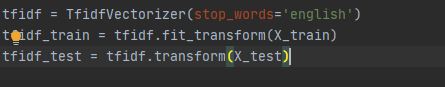
\includegraphics[scale=0.6]{fig/4.PNG}
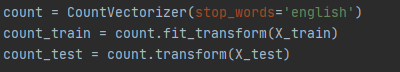
\includegraphics[scale=0.7]{fig/5.PNG}
\bigskip
\subsection{Initialize and Compare Models}
\subsubsection{MultinomialNB()}
Firstly, I used MultinomialNB(). The multinomial Naive Bayes classifier is suitable for classification with discrete features(For Example, Word counts for text classification). I implemented using TfidfVectorizer and CountVectorizer to see difference. Using fit(), I fit my data and predict() to estimate. To see difference and efficient, I need to see accuracy score and for this I used "accuracy\_score" and "plot\_confusion\_matrix" confusion matrix and visualization
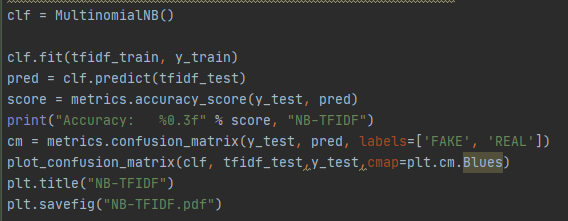
\includegraphics[scale=0.7]{fig/6.PNG}\bigskip\newline
\noindent
When I look the output;\newline
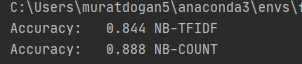
\includegraphics[scale=0.7]{fig/7.PNG}\newline
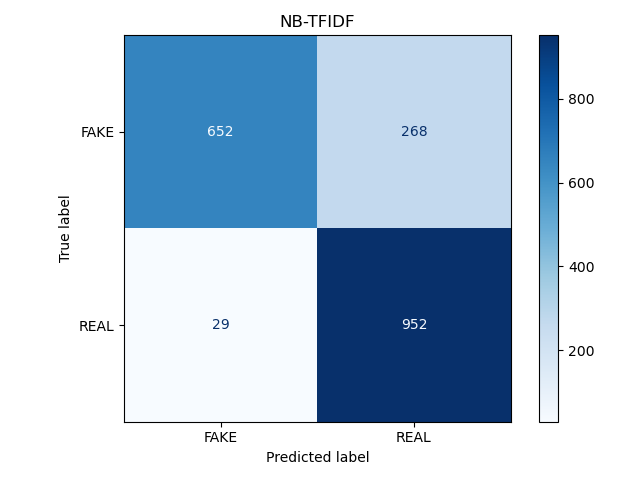
\includegraphics[scale=0.3]{fig/8.PNG}
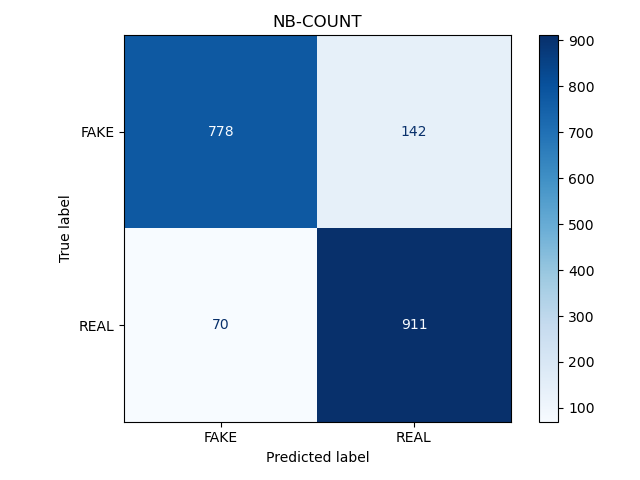
\includegraphics[scale=0.3]{fig/9.PNG}
\bigskip\newline
\noindent
I determined countVectorizer works better than tfidtVectorizer. Because Naive Bayes requires integer feature counts. CountVectorizer() returns ints.
\subsubsection{PassiveAggressiveClassifier()}
Passive-aggressive classification is one of the available incremental learning algorithms and it is very simple to implement. I implemented using TfidfVectorizer and CountVectorizer to see difference. Using fit(), I fit my data and predict() to estimate. To see difference and efficient, I need to see accuracy score and for this I used "accuracy\_score" and "plot\_confusion\_matrix" confusion matrix and visualization\newline
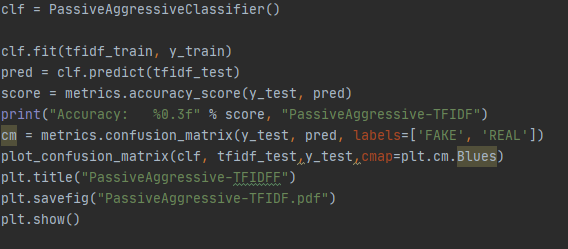
\includegraphics[scale=0.7]{fig/10.PNG}\bigskip\newline
\noindent
When I look the output;\newline
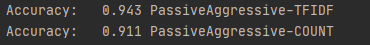
\includegraphics[scale=0.7]{fig/13.PNG}\newline
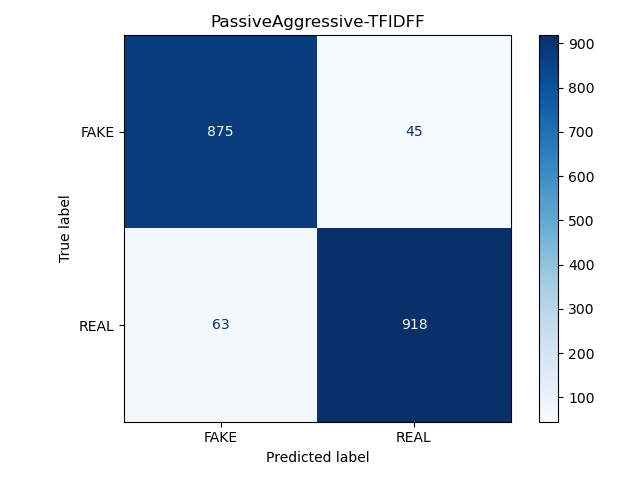
\includegraphics[scale=0.3]{fig/16.PNG}
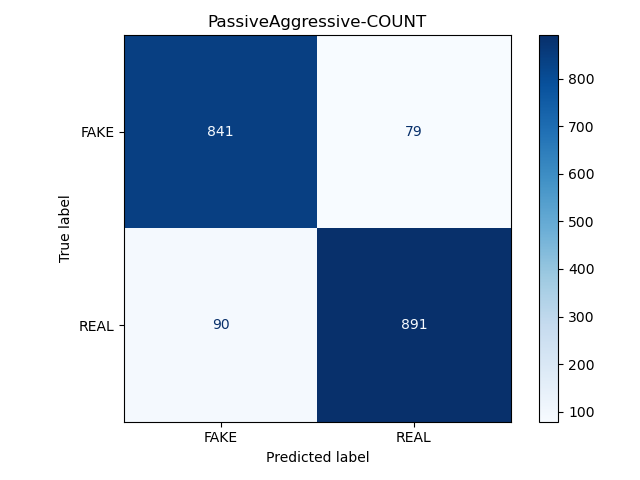
\includegraphics[scale=0.3]{fig/12.PNG}
\bigskip\newline
\noindent
As we see to confusion matrices and accuracy scores, PassiveAgressive works better than NB. But differently from NB, TFIDF works better than Count in PassiveAgressive. Finally, I got 0.943 accuracy.


\section{Results}
I observed how to think up a algorithm for fake news detection. As seen below, Fake news generally includes political words\newline
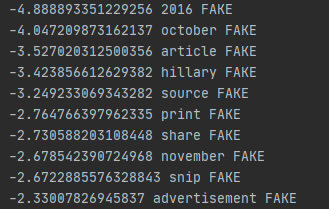
\includegraphics[scale=0.6]{fig/15.PNG}



\section{Conclusion}
In conclusion, Everything can handle with data processing. In this project, I worked on news. Are news fake news or not? This is the project goal. I used vectorizers to split text to words. There are 3 types vectorizers. TFIDFVectorizer and CountVectorizer is the most useful vectorizers. After that, I used some classifier suitable to text classifier projects. Lastly, I visualized data and results.


\nocite{*}
\bibliographystyle{plain}
\end{document}

